\documentclass[
  a4paper,            % DIN A4
  DIV=10,             % Schriftgröße und Satzspiegel
  oneside,            % einseitiger Druck
  BCOR=5mm,           % Bindungskorrektur
  parskip=half,       % Halber Abstand zwischen Absätzen
  numbers=noenddot,   % Kein Punkt hinter Kapitelnummern
  bibliography=totoc,  % Literaturverzeichnis im Inhaltsverzeichnis
  listof=totoc,       % Abbildungs- und Tabellenverzeichnis im Inhaltsverzeichnis
  table
]{scrreprt}
\usepackage{../style/thesisstyle}

\newcommand{\q}[1]{\glqq{}#1\grqq{}}

\makeglossaries           % create all glossary entries (remember: run makeglossaries manually)
\loadglsentries{thesisglossaries.tex}  % load acronym, symbol and glossary entries

\sisetup{locale = DE}     % siunitx locale setup
%\DeclareSIUnit \fps{fps}  % a custom unit (usage: \SI{24}{\fps})

\begin{document}
% !TEX root = ../thesis.tex
%
% configurations
%

% English Language support
% -> uncomment if needed
% Beta!
%\fullenglish{yes}
\fullenglish{no}

% text field
%-> replace supervisor names with correct ones
\firstSupervisor{Prof. Dr. Stefan Sarstedt}
\secondSupervisor{Prof. Dr.-Ing. Lars Hamann}

% text field
%-> replace title with your thesis title
\thesisTitle{Erhöhung der Korrektheit des States in Frontend Webapplikationen mit Strikten Übergängen}
% TODO Title knapper schreiben
\thesisTitleEN{Increasing Correctness in State of Frontend Web Applications with Strict Transitions}

% text field
%-> replace the key words with your own key words
\keywordsDE{State-Management, Webapplikationen, Frontend}
\keywordsEN{State Management, Web Applications, Frontend}

% text field
%-> replace the text with a description of the thesis
\abstractDE{Frontend-Applikationen sind ein wesentlicher Bestandteil jeder Webapplikation und sind für Teile der Geschäftslogik und die UI verantwortlich. Steigende Anforderungen in Geschwindigkeit, Responsiveness und Features erhöhen die Komplexität enorm. Um einen Teil dieser Komplexität zu verwalten, kommen \acrlong{ac:sm}-Lösungen zum Einsatz. Diese übernehmen wichtige Aufgaben wie beispielsweise das Data-Fetching, die Datentransformation und die Datenspeicherung. Fehler im State können daher einen verhältnismäßig großen Einfluss auf das Nutzererlebnis und das operative Geschäft haben. Damit Fehler und Defekte in diesem Bereich reduziert und schnell erkannt werden, wird eine strikte Erweiterung für \acrlong{ac:sm} im Allgemeinen vorgestellt und mit dem normalen Ansatz verglichen.}
\abstractEN{Frontend applications are an essential part of any web application and are responsible for parts of the business logic and the UI. Increasing demands for speed, responsiveness, and features significantly raise complexity. To manage part of this complexity, state management solutions are used. These handle important tasks such as data fetching, data transformation, and data storage. Errors in the state can, therefore, have a relatively large impact on the user experience and operational business. To reduce and quickly detect errors and defects in this area, a strict extension for state management, in general, is introduced and compared to the conventional approach. A reduction in error-proneness as well as improvements in developer experience, readability, and maintainability are considered plausible, even though these aspects could not be definitively proven within the scope of the study.}

% text field
%-> replace john with your name
\thesisAuthor{Soheil Nazari}

% text field
%-> enter the submission date
% TODO UPDATE THIS
\submissionDate{03. März 2025}

% switch - uncomment only one
%-> uncomment NDA or public
%\NDA{yes}
\NDA{no}

% switch - uncomment only one
%-> uncomment old standard cover or cover Corporate Design 2017
\Cover{CD2017}
%\Cover{CD2017NoLogo}
%\Cover{Std2018}
%\Cover{Std2018_green} 			% with green bar

% switch - uncomment only one
%-> uncomment to show list of figures or not
\ListOfFigures{yes}
%\ListOfFigures{no}

% switch - uncomment only one
%-> uncomment to show list of tables or not
\ListOfTables{yes}
%\ListOfTables{no}

% switch - uncomment only one
%-> uncomment to show list of accronyms or not
\ListOfAccronyms{yes}
%\ListOfAccronyms{no}

% switch - uncomment only one
%-> uncomment to show list of symbols or not
\ListOfSymbols{yes}
%\ListOfSymbols{no}

% switch - uncomment only one
%-> uncomment to show list of glossary entries or not
\Glossary{yes}
%\Glossary{no}

% switch - uncomment only one
%-> uncomment the study course you are in
%\studycourse{ITS}
%\studycourse{TI}
%\studycourse{AI}
\studycourse{WI}
%\studycourse{EI}
%\studycourse{REE}
%\studycourse{BMP}		
%\studycourse{BMP-hp}	 % Internship Report in M&P
%\studycourse{BMT}
%\studycourse{BMT-st}    % Study / home assignment in BMT
%\studycourse{BMT-hp}    % Internship Report in BMT
%\studycourse{MI}
%\studycourse{MIK}
%\studycourse{MA}
    % load all settings

\hyphenation{Ba-che-lor-the-sis Mas-ter-the-sis}

% Cover page here, no page number
\ICoverPage

% PDF Metadata
% !TEX root = ../thesis.tex
%
% PDF Metadata integration
% @author Thomas Lehmann
%

% PDF Metadata
\hypersetup{
pdftitle={\IthesisTitle},
pdfauthor={\IthesisAuthor},
pdfkeywords={\IkeyWordsEN}
}

% Titlepage is page one even if the number is not shown.
\pagenumbering{roman}
% Title page here
% !TEX root = ../thesis.tex
%
% title page
% @author Thomas Lehmann
% Hints for title page and page numbering: https://en.wikipedia.org/wiki/Title_page
%
\title{\IthesisTitle}   % set latex default title to be used by hyperref in pdf
\author{\IthesisAuthor} % set latex default author to be used by hyperref in pdf

\newpage
\thispagestyle{empty}
{\fontfamily{phv}\selectfont
  \hfuzz=20pt       % suppress warnings due to extension onto page margins

  % Author of thesis
  \vspace*{1cm}
  \begin{minipage}[b]{\textwidth}
    \fontsize{14pt}{20pt}
    \selectfont
    \begin{center}
      \IthesisAuthor
    \end{center}
  \end{minipage}

  % Title of thesis
  \vspace{1.5cm}
  \begin{minipage}[b][0cm][t]{\textwidth}
    \fontsize{18pt}{20pt}
    \selectfont
    \begin{center}
      \IthesisTitle
    \end{center}
  \end{minipage}

  % Important information
  \begin{textblock*}{\textwidth}(40mm,210mm)
    \begin{minipage}[b]{\textwidth}
      \hbadness=10001    % suppress underfull warning due to short text
      \fontfamily{cmr}\selectfont
      \fontsize{12pt}{14pt}
      \selectfont
      \ifdefined\ILanguageEN
        \IthesisKindEN ~submitted for examination in \IthesisExaminationEN \\
        in the study course \textit{\IstudyCourseName} \\
        at the \IthesisDepartmentFullEN \\
        at the \IthesisFacultyFullEN \\
        at University of Applied Science Hamburg\\

        Supervisor: \IfirstSv \\
        \ifdefined\IisTermPaper
          % left blank
        \else
          \ifdefined\IisInternshipReport
	  Supervised: \IsecondSv\\
          \else
        Supervisor: \IsecondSv \\
          \fi\fi
        
        Submitted on: \ISubDate \\
      \else
      	\ifdefined\IisInternshipReport
        \IthesisKindDE ~eingereicht im Rahmen des \IthesisExaminationDE \\	
	\else
        \IthesisKindDE ~eingereicht im Rahmen der \IthesisExaminationDE \\
        \fi
	im Studiengang \textit{\IstudyCourseName} \\
        am \IthesisDepartmentFull \\
        der \IthesisFacultyFull \\
        der Hochschule für Angewandte Wissenschaften Hamburg\\

        Betreuender Prüfer: \IfirstSv \\
        \ifdefined\IisTermPaper
          % left blank
        \else
          \ifdefined\IisInternshipReport
        betriebliche Betreuung: \IsecondSv \\							
	  \else
        Zweitgutachter: \IsecondSv \\
        \fi\fi

        Eingereicht am: \ISubDate \\
      \fi
    \end{minipage}
  \end{textblock*}
}


% Abstract page here
% !TEX root = ../thesis.tex
%
% abstract page
% @author Thomas Lehmann
%
\newpage
\thispagestyle{plain}
\clearpage
\hfuzz=12pt       % suppress warnings due to extenstion onto page margins

\textbf{\IthesisAuthor}

\vspace{0.3cm}
\textbf{Thema der Arbeit}

\IthesisTitle

\vspace{0.3cm}
\textbf{Stichworte}

\IkeyWordsDE

\vspace{0.3cm}
\textbf{Kurzzusammenfassung}

\begin{minipage}{\textwidth}
\IabstractDE
\end{minipage}

\vspace{1.0cm}
\textbf{\IthesisAuthor}

\vspace{0.3cm}
\textbf{Title of Thesis}

\IthesisTitleEN

\vspace{0.3cm}
\textbf{Keywords}

\begin{minipage}{\textwidth}
\IkeyWordsEN
\end{minipage}

\vspace{0.3cm}
\textbf{Abstract}

\IabstractEN


% Table of contents here
\tableofcontents

% List of figures here
\IListOfFigures

% List of tables here
\IListOfTables

% List of accronyms here
\IListOfAccronyms

% List of symbols here
\IListOfSymbols

% Uncomment if list of source code is needed (rarely).
%\lstlistoflistings  % requires package listings, needs to uncommenting of usepackage

% path to the chapters folder is set to find the images used there
\graphicspath{ {./chapters/} }

% Chapters
\clearpage
\pagenumbering{arabic}
\chapter{Einleitung}

\section{Die Rolle des State-Managements in Frontend Webapplikationen}

Moderne Webapplikationen folgen der Komponenten-Architektur. Verschiedene Komponenten können von den selben Daten abhängig sein. Die Daten werden in der Regel während der Lebensdauer der Browser-Session basierend auf Interaktionen des Benutzers aktualisiert und erweitert. Änderungen in den Daten müssen den betroffenen Komponenten mitgeteilt werden. In einigen Fällen ist die Synchronisierung der Daten im Frontend mit den Daten des Servers erforderlich. Um HTTP Aufrufe zu sparen, können verschiedene Mechanismen, wie beispielsweise Caching oder Debouncing verwendet werden. Diese Faktoren erhöhen, die ohnehin schon hohe Komplexität und Fehleranfälligkeit zusätzlich.

Um diese Komplexität effizient zu verwalten, werden State-Management Lösungen wie Redux \cite{redux}, NgRx \cite{ngrx} oder Pinia \cite{pinia} verwendet. Mit Hilfe dieser Open Source JavaScript Bibliotheken, können Daten beim Bedarf von einer API abgerufen, transformiert und im Speicher gespeichert werden. Die meisten State-Management Bibliotheken sind eng mit einem UI-Framework gekoppelt. \cite{ui-frameworks-and-state-management}. Aus diesem Grund sind sie ein fundamentaler Baustein jeder größeren Frontend Webapplikation.

\section{Ziel dieser Arbeit}

Mit der Komplexität erhöht sich auch die Fehleranfälligkeit. Fehler im Zustand, also Daten der Applikation, haben einen direkten Einfluss auf das Angezeigte. Wenn die Applikation sich in einem "falschen" Zustand befindet und es keine Laufzeitfehler gab, können die Verantwortlichen (in der Regel, die Entwickler) unter Umständen, nicht darüber informiert sein. Dies führt zu langlebigen Bugs.

Ziel dieser Arbeit ist es, einen Ansatz zu erarbeiten, bei dem die Möglichkeit eines Befindens in einem "falschen" oder "illegalem" Zustand eliminiert wird. Dazu wird jeder zusammenhänge Teil des Zustands als ein endlicher Automat \cite{fa} abgebildet. Dahingehend wird jede Änderung in diesem Zustand wie ein Übergang bei einem endlichen Automaten behandelt. Es wird vorgeschlagen die beliebten State-Management Lösungen um "strikte" Übergänge, wie bei einem DFA, zu erweitern. Auf diesem Wege wird eine Reduzierung von Bugs in größeren Applikationen bestrebt. Dabei wird insbesondere auf die Lesbarkeit und Wartbarkeit des Quellcodes und die Developer Experience geachtet.
\chapter{Methodologie}

TODO 

\section{Code Ausschnitte}

TypeScript wird benutzt um, Aufbau von Objekten oder Funktionen zu beschreiben. Längere Strukturen werden mit Hilfe von Code-Bespielen veranschaulicht. Hierfür wird ebenfalls TypeScript verwendet. An viele Stellen wird auf Type-Annotationen verzichtet, damit die Beispiele leicht lesbar bleiben.
\chapter{State-Management Ansätze} \label{sm-ansaetze}

Bei den populären \acrshort{ac:sm}-Lösungen folgt Redux und NgRx dem Flux-Pattern\cite{historyOfRedux}\cite{ngrxGettingStarted}, wobei Zustand und Pinia einen anderen, Framework-nahen Ansatz verfolgen. Im Folgenden wird die Funktionsweise und die Eigenschaften von Redux und Pinia näher beschrieben. Da diese grundlegend unterschiedliche Ansätze verfolgen und andere \acrshort{ac:sm}-Lösungen sich einem der beiden ähneln.

\section{Redux}

Redux definiert sich durch folgenden vier Eigenschaften:
\begin{enumerate}
  \item Unveränderlichkeit (Immutability): Änderung am State sind ausschließlich über die APIs von Redux unter Beachtung der Unveränderlichkeit möglich.
  \item Zentralisierung des Zustandes: Der gesamte Applikationszustand lebt in einem zentralen \acrlong{ac:js} Objekt.
  \item Nachvollzierbarkeit (Traceability): Während der gesamten Lebensdauer der Applikation, sind Änderungen am Zustand auf deren Ursprung verfolgbar.
  \item Event basiert: Es wird das Beobachter-Muster (Observer Pattern) verwendet.
\end{enumerate}

Das Verhalten des Stores wird durch \textit{actions} und \textit{reducer} definiert.
% Außerdem können optionale \textit{selectors} benutzt werden um aus bestimmten Teilen des Zustandes zu lesen.

\subsection{Actions}

Eine Aktion (Action) beschreibt eine Änderung oder Interaktion in und mit der Applikation. Beispielsweise könnte eine \textit{counter-clicked} Action versendet (dispatch) werden, wenn der Nutzer auf den \textit{Zähler erhöhen} Button drückt. Oder, wenn der Nutzer sich erfolgreich angemeldet hat, kann eine entsprechende Action versendet werden. Intern ist eine Action ein \acrshort{ac:pojo}.\cite{reduxStateActionReducers}

Es wird folgende Struktur für Actions empfohlen:
\begin{lstlisting}
type Action<T> = {
  type: string,
  payload?: T
}
\end{lstlisting}

Das Feld \textit{type} beschreibt die Action und das optionale Feld \textit{payload} enthält weiterführende Daten.

\subsection{Reducer}

Ein Reducer ist für die Initialisierung und Aktualisierung des Zustandes zuständig. Ein Reducer wird als eine Pure-Function mit zwei Parametern definiert.
Der erste Parameter ist das Zustandsobjekt und der zweite die versendete Action. Der Rückgabewert dieser Funktion ist das neue Zustandsobjekt. Da es sich hier um eine Pure-Funtion handelt, dürfen es hier keine Seiteneffekte stattfinden. Wie anfangserwähnt, ist der Zustand Unveränderlich, daher dürfen hier keine direkten Veränderungen des Zustandes stattfinden. Es wird lediglich ein neues Objekt zurückgegeben. Fall es keine Veränderungen stattfinden sollen, kann das ursprüngliche Objekt aus dem ersten Parameter unverändert zurückgegeben werden.\cite{reduxStateActionReducers}

Es wird folgende Struktur für Reducer empfohlen:
\begin{lstlisting}
type Reducer<S, A> = (state: S, action: A) => S
\end{lstlisting}

Beispiel reducer:

\begin{lstlisting}
function reducer(state = { user: null }, action) {
  switch (action.type) {
    case 'user-logged-in':
      return {
        ...state,
        user: {
          userId: action.payload.userId
        },
      }
    case 'user-logged-out':
      return {
        ...state,
        user: null,
      }
    default:
      return state
  }
}
\end{lstlisting}

Es wird die \textit{Spread Syntax: ...} aus ECMAScript 6 genutzt, um as ursprüngliche Zustandsobjekt zu klonen.\cite{mdnSpreadSyntax}

\subsection{Definition und Interaktion mit dem Store}

Der Store wird mit Hilfe der \textit{createStore} API erstellt. Als Parameter wird die Reducer-Function übergeben. Der Rückgabewert ist das Store-Objekt. Dieses bietet Zugang zu unteranderem \textit{dispatch} und \textit{getState} Methoden. Mit diesen kann jeweils Actions versendet und aus dem Store gelesen werden.

\begin{lstlisting}
import { createStore } from 'redux'

const store = createStore(reducer)
store.dispatch(action)
const user = store.getState().user
\end{lstlisting}

\begin{figure}[H]
  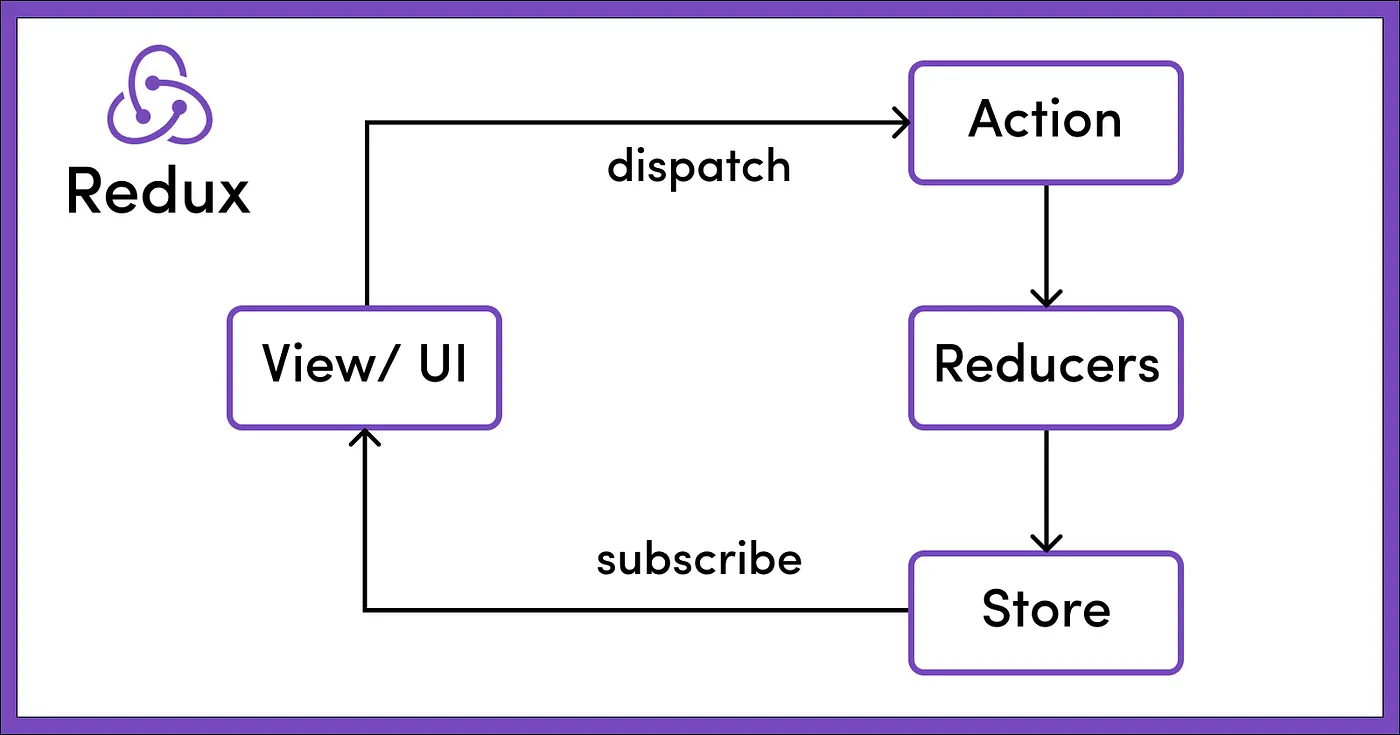
\includegraphics[width=1\textwidth]{redux-lifecycle.png}
  \caption{Redux Datenfluss}
  \label{fig:redux-lifecycle}
\end{figure}

\section{Pinia}

Pinia ist sehr eng gekoppelt mit dem Vue Framework und nutzt dessen Mechanismen der Reaktivität zu Datenhaltung. Das führt dazu, dass Pinia selbst minimal bleibt und die Daten ohne weiteres reaktiv sind. Im Gegensatz zu Redux und NgRx setzt diese Store-Lösung nicht das Flux-Pattern um. Dank dieser Praxis, ist weniger Code nötig um einen Store zu definieren. Außerdem folgt Pinia nicht den Single-Store-Ansatz, bei dem alle Daten in einem zentralen Objekt leben. Sondern sind für Teile der Daten eigenständige Store-Instanzen zuständig. Pinia bietet zwei verschiedene APIs zu Definition von Stores an. In dieser Arbeit wird die \textit{Options API} verwendet. Die Konzepte lassen sich auch auf die \textit{Composition API} übertragen.\cite{piniaDefiningAStore} Die zwei essentiellen Konzepte sind \textit{State} und \textit{Action}.

\subsection{State}

State ist eine Funktion, die ein Objekt zurückgibt. Dieses enthält den Zustand. 

\subsection{Action}

Eine Action ist eine Methode, die den State verändert und in einem \textit{actions} Objekt definiert wird.

\subsection{Definition eines Stores}

Zu Definition eines Stores wird die \textit{defineStore} API genutzt. Als Parameter wird ein eindeutiger Name und eine Beschreibung des Stores in Form eines Objekts übergeben. In dem zweiten Paramter werden die Felder \textit{state} und \textit{actions} definiert.

\begin{lstlisting}
const useUserStore = defineStore('user-store', {
  state: () => {
    user: null
  },
  actions: {
    updateUser(newUser) {
      this.user = newUser
    }
  }
})
\end{lstlisting}

Auf die Felder in dem State-Objekt wird in einer Action mit \textit{this} zugegriffen. Das State-Objekt wird seitens Pinia intern jeder Action gebunden.

\subsection{Interaktion mit dem Store}

Der Store kann in einer belibiegen Vue-Komponente importiert werden. Die Felder des Objekts, das von der state Funktion zurückgegeben wird, werden automatisch zu Feldern des Store Objekts. Genauso werden auch die Methoden des Actions-Objekts auch zu Member des Store Objekts.

\begin{lstlisting}
  const userStore = useUserStore()
  
  // userStore.user
  // userStore.updateUser
\end{lstlisting}

Die State im oberen Beipiel ist reaktiv und kann als \textit{userStore.user} im Template der Komponente referenziert werden. Die Desktrukturierung (destructuring) des Store-Objekts, im oberen Beispiel \textit{userStore}, führt zur Verlust der Reaktivität. Aus diesem Grund wird die Punktnotation empfohlen.\cite{piniaDefiningAStore}

% Add additional chapters here

%\bibliographystyle{plain}
\bibliographystyle{dinat}
\bibliography{literature}

% Appendix
\appendix
% !TEX root = ../thesis.tex
% appendix example chapter
% @author Thomas Lehmann
%

\chapter{Anhang}

\section{Verwendete Hilfsmittel}
In der Tabelle \ref{tab:tooling} sind die im Rahmen der Bearbeitung des Themas der \IthesisKindDE~verwendeten Werkzeuge und Hilfsmittel aufgelistet.

\begin{table}[h!]
\caption{Verwendete Hilfsmittel und Werkzeuge}
\begin{tabular}{|l|l|}
\hline 
\rowcolor{lightgray} Tool & Verwendung \\
\hline
\LaTeX & Textsatz- und Layout-Werkzeug verwendet zur Erstellung dieses Dokuments \\
\hline
 & \\
\hline
\end{tabular}
\label{tab:tooling}
\end{table}



\IGlossary

\Istatement

\end{document}
